%% Hanford investigations

%% TCS schematic for LIGO Hanford for O3
%% TCS pre-loading
 %% Current methodology for tuning TCS
  %% Detail Hanford's methods
 %% Increasing RH tuning speed


%As shown in Chapter 1,  increasing input power leads to a direct increase to the sensitivity of a DRFPMI to make gravitational wave detections. But one implication of this is the necessity for thermal compensation. As the interferometer increases input power, you directly couple more light into the Fabry-P\'{e}rot cavity arms; and even with optics ultra-low absorption ($\approx 400 \; \mathrm{ppb} \pm 150 \; \mathrm{ppb}$ \textcolor{red}{alog ? or point absorber paper}) still induce thermo-optic effects with the projected circulating arm power of 200 kW. A symptom of this is mode mismatch throughout the interferometer, a problem that contributes to loss of usable optical power throughought the DRFPMI which can reduce sensitivity two-fold: loss of power to your readout, and reduced efficacy of the current solution to reduce the quantum noise limit (squeezing).

During O3a circulating arm power at the LIGO Hanford observatory reached beyond 180 kW; emphasizing importance on properly tuned thermal compensation is in O3 to avert arm cavity mode mismatch. Detailed in this chapter is a summary of related comissioning efforts at LHO including but not exclusive to: citations of the initial computed O3 TCS pre-load, the development and implementation of real-time digital filtering for improved ring heater actuation response by a factor of $\approx 6$, and the impacts of high absorption points aka point absorbers discovered on arm cavity test masses along with the inital efforts to mitigate them. 

\section{A priori TCS pre-load methodology for O3a}
Preserving the nominal 50km test mass ROC (as well as cavity resonance) requires countering the positive thermal lens induced by high circulating interferometer arm cavity power. Preparing for the central uniform test mass distortion from the carrier requires well established thermal actuator settings which in turn inform of how to `pre-load' the TCS actuators based on early estimates of test mass absorption. Initial order of magnitude estimates of the wavefront distortion from ultra-low absorption fused silica test mass under the influence of a centered high power gaussian beam as well as annular ring heater actuation are available \cite{hello_vinet, Ramette:16}; though variations of the absorption between any two test mass mirrors calibrated defocus measurements using the Hartmann wavefront sensors \textcolor{red}{sensitive to auxilary beams imaged onto the test mass mirror surfaces}. The measured wavefront distortion is then mapped in real time to Zernike polynomial coefficients used to compute the differential thermal lens in diopters. 

\subsection{The thermo-optic response}
\begin{figure}[!h]
  \centering
  \begin{subcaptiongroup}
	  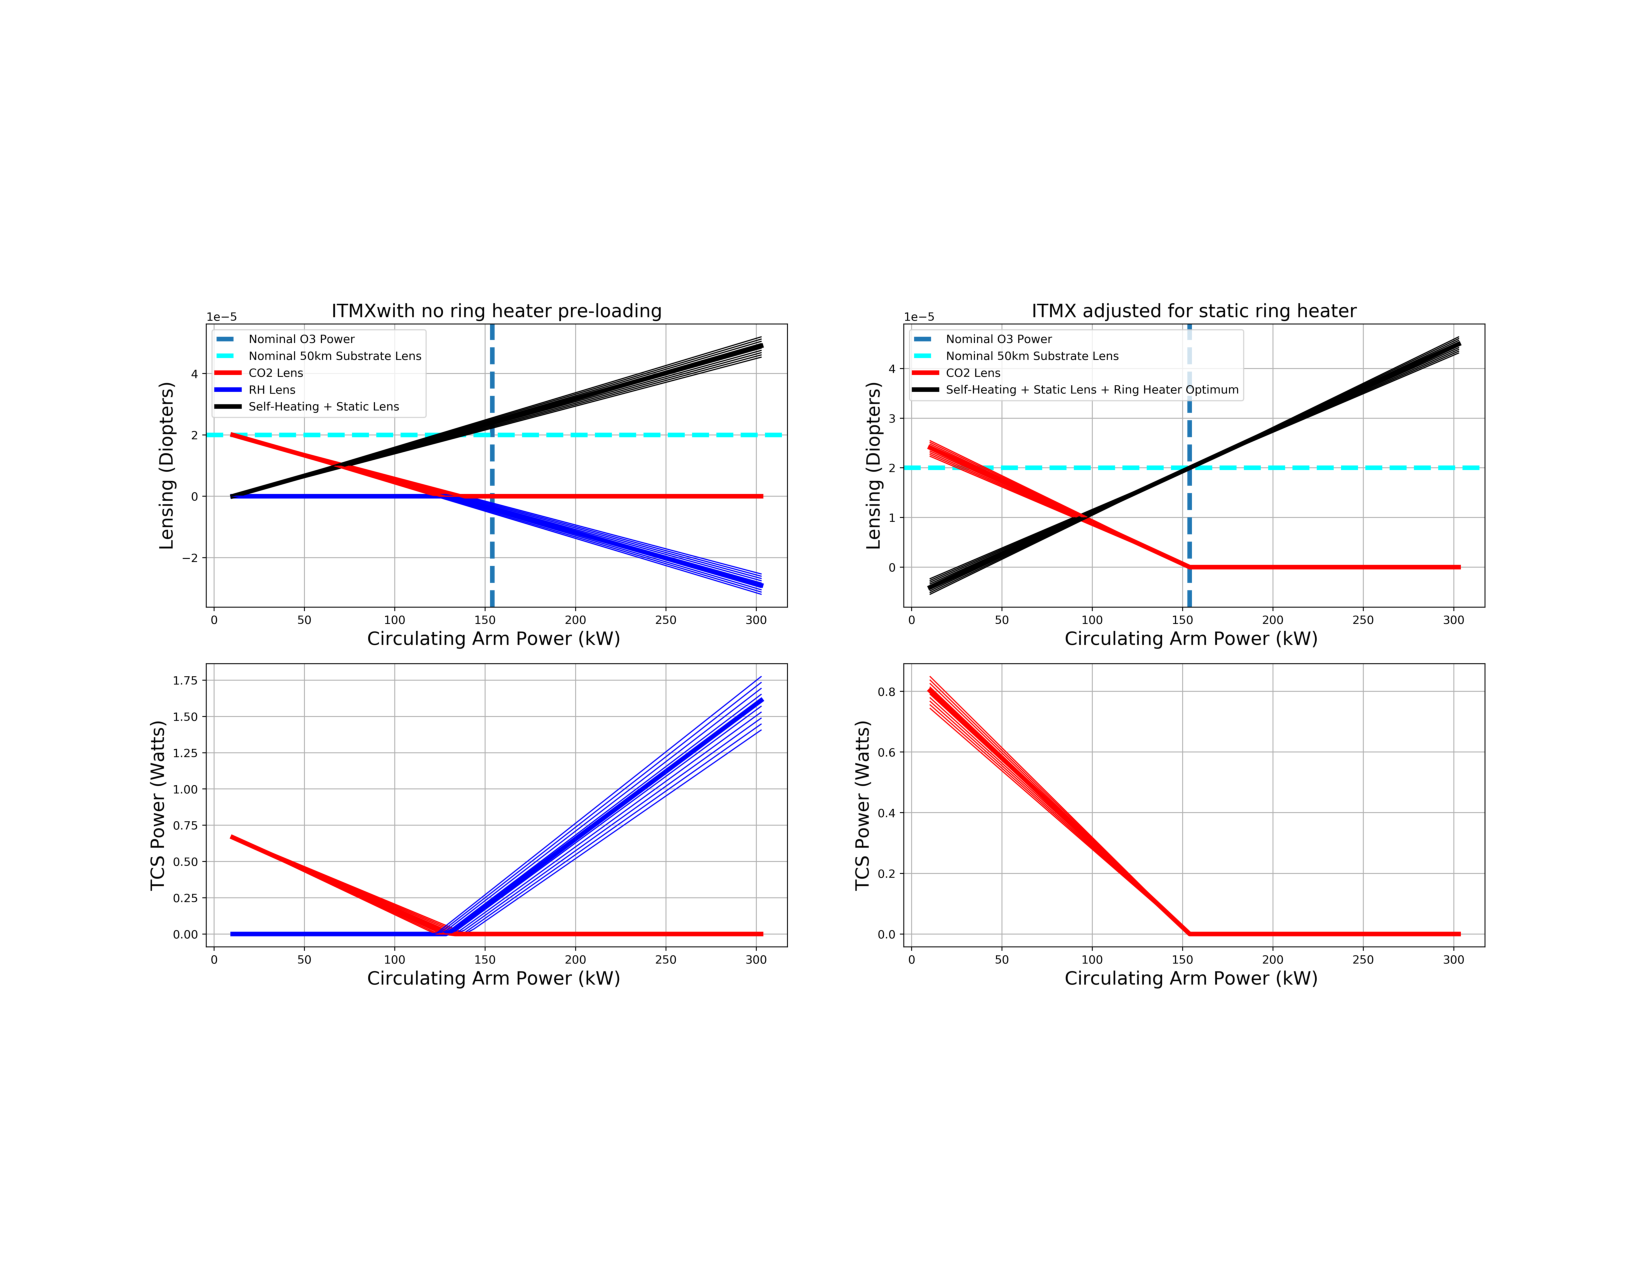
\includegraphics[width=\textwidth]{TCS/ITMX_TCS_Settings_tvo.pdf}
	  \phantomcaption\label{ITMX_TCS}
  \end{subcaptiongroup}
  \captionsetup{subrefformat=parens}
  \hfill
  \caption{Observed thermo-optic responses from the carrier beam self heating and TCS actuation (central CO2 laser heating and annular ring heating.)} 
\label{fig:thermooptic_response}
\end{figure}
Although the thermo-optic time constant for central self-heating response is demonstrably different from annular ring heating, it is similar to that seen from central CO2 actuation. Because of this, LHO applies the central CO2 heating and static annular ring heating to a power level that respectively mimics and actuates for projected thermal deformation from the circulating high power resonant carrier beam in the Fabry-Perot arm cavities. Once the DRFPMI coupled cavities are configured or ``locked'', the input carrier power is gradually increased while simultaneously decreasing CO2 laser power, in order to mitigate the differential thermo-optic responses from the arm cavity test masses when reaching maximum power.
\begin{figure}[!h]
  \centering
  \begin{subcaptiongroup}
	  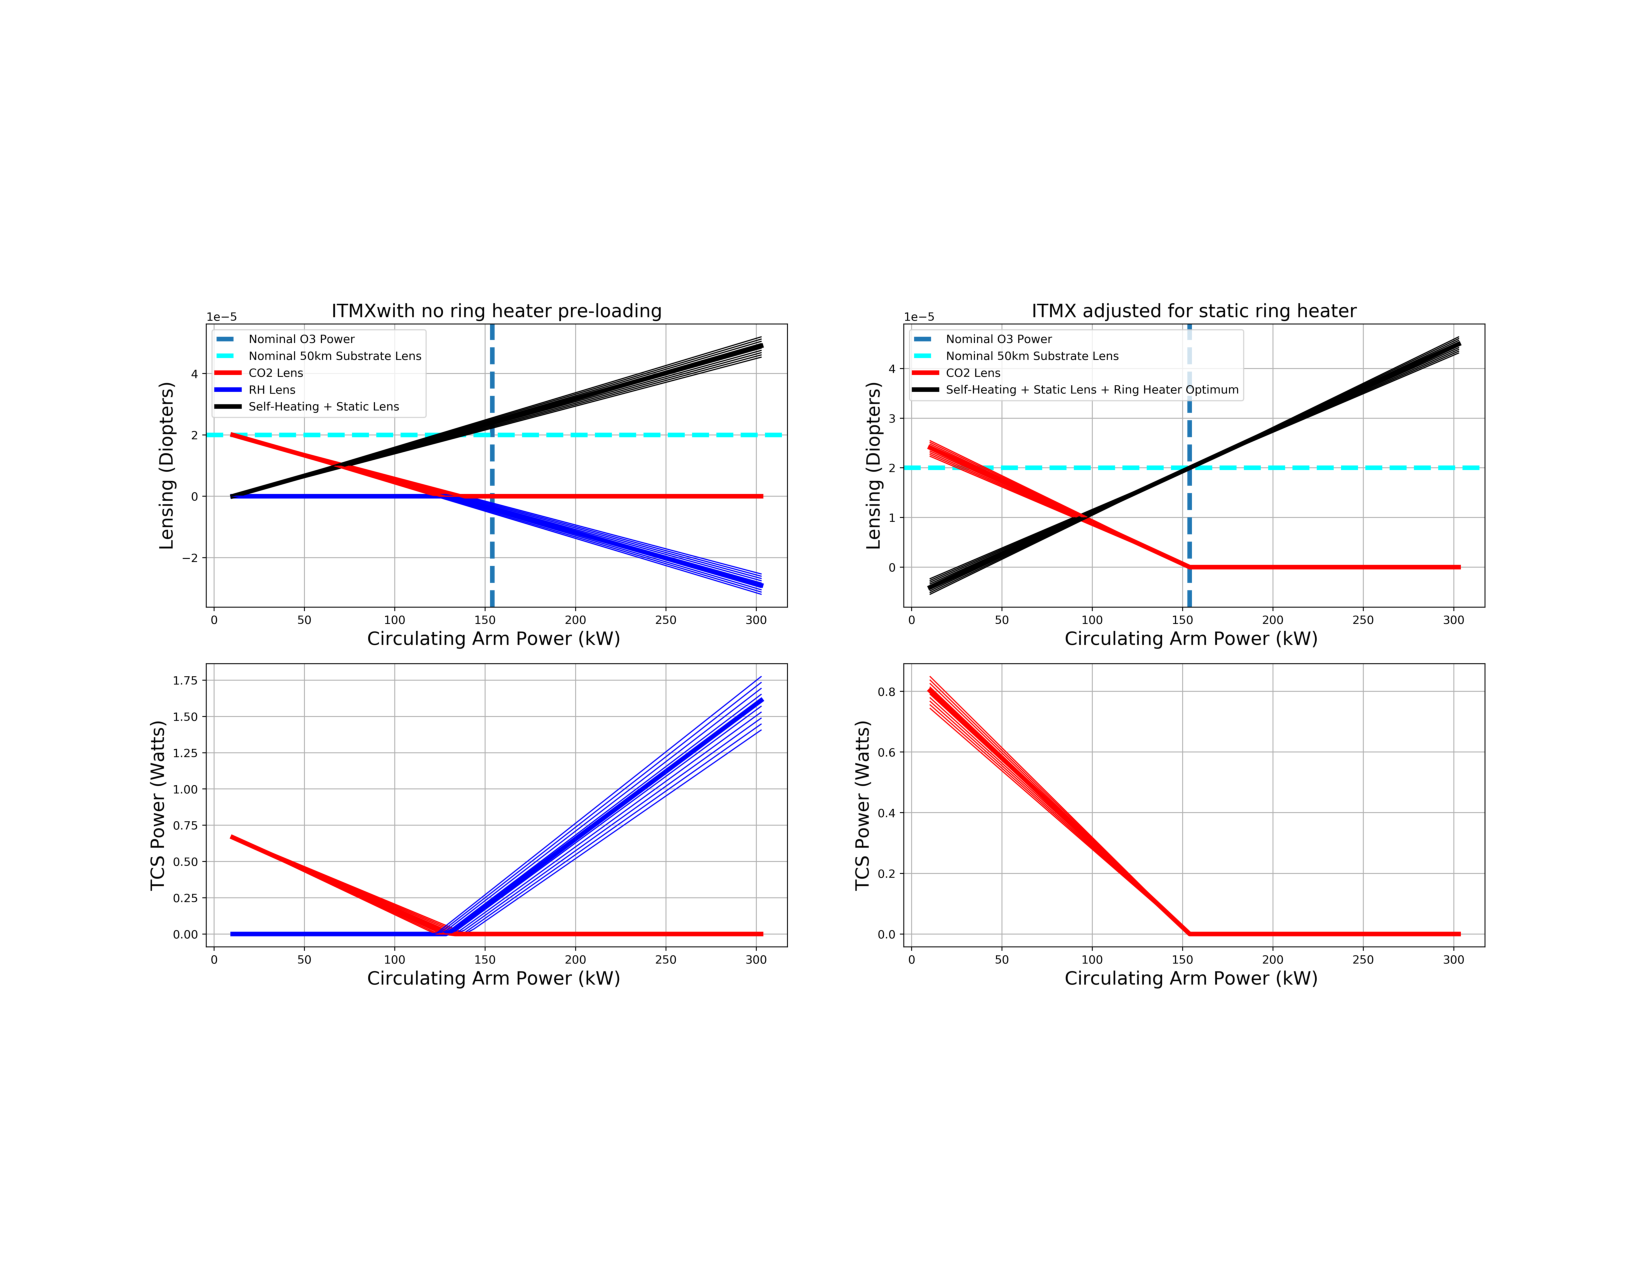
\includegraphics[width=\textwidth]{TCS/ITMX_TCS_Settings_tvo.pdf}
	  \phantomcaption\label{ITMX_TCS}
	  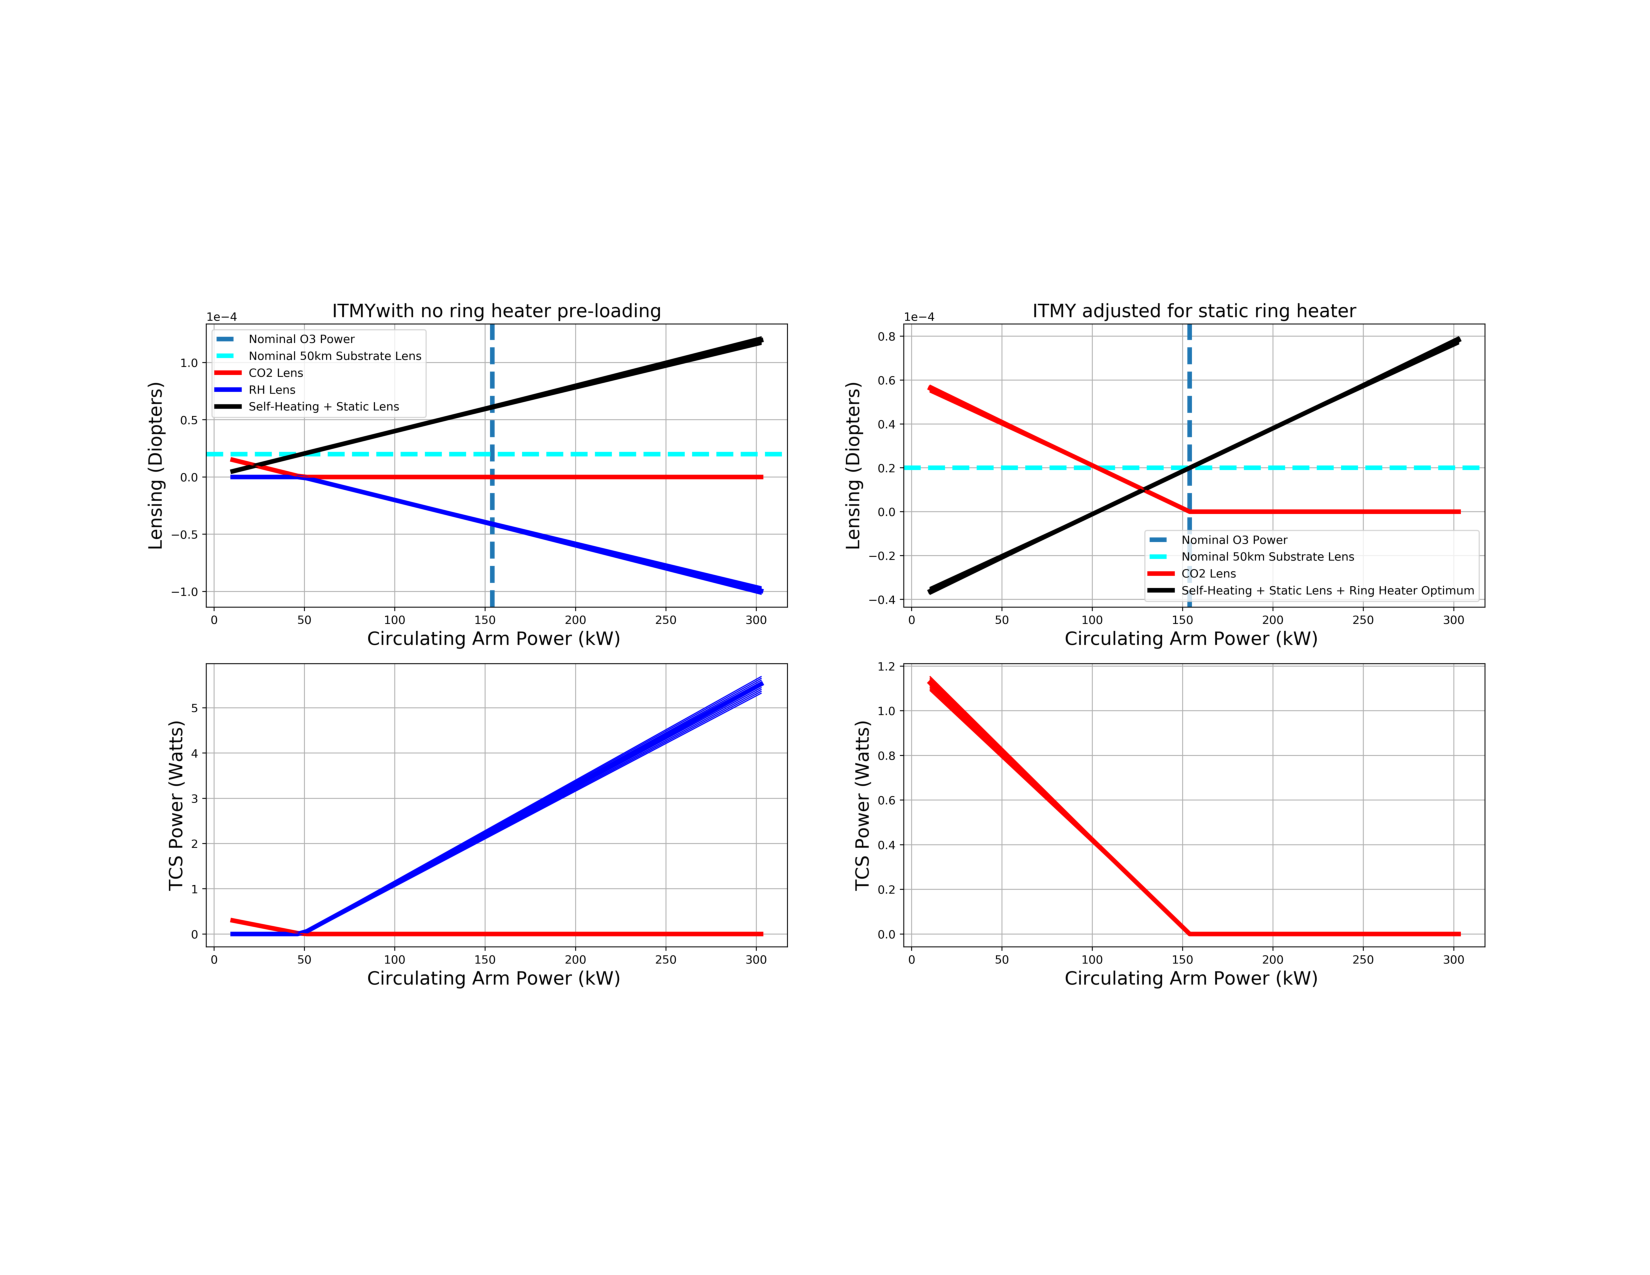
\includegraphics[width=\textwidth]{TCS/ITMY_TCS_Settings_tvo.pdf}
	  \phantomcaption\label{ITMY_TCS}
  \end{subcaptiongroup}
  \captionsetup{subrefformat=parens}
  \hfill
  \caption{The initial pre-load estimates for the ITMs at the LIGO Hanford Observatory for O3a as provided in \cite{tvo}} 
  \label{fig:O3_preload_tvo}
\end{figure}


\section{A posteriori thermal compensation for O3a}
While approaching designed arm cavity power, the presence of non-uniform absorption on the test mass coating surface called for significant deviation from the original pre-loading algorithm. Assessment of the situation to inform of any improvements in detector sensitivity requires an initial characterization of these high absorbtion points; noting the characteristic optical path distortion as measured on the Hartmann wavefront sensors and the impacts on interferometer operations especially at high power. Current thermal actuation solutions are currently designed to control the TEM00 beam waist size and location though modifications to the CO2 laser actuator were attempted. Summary of the findings indicates that these absorbers may impose a barrier to maintaining high power in the arm cavities if proactive measures are not sufficient in avoiding them; whether they are a result of preventable surface particulates or improved higher frequency.  

%The presence of high absorption points on the test masses (aka point absorbers) required adjustments to the TCS pre-load and various ring heater and CO2 settings were sampled. Part of this sampling lead to the development of a input ring heater filter allowing actuation to reach ? percent of the desired optical power within 2 hours compared to the 12 hour response pre-filter. Higher spatial frequency actuation in the form of a CO2 mask was also tried.

\subsection{Point absorbers in O3a}
\textcolor{red}{A summary of the found absorbers \\
	* Insert optical path distortion photos (taken using Dan's software too) \\
		* ITMY absorbers \\
		* ETM absorbers \\
	* Reference Aidan's paper} \\

Impact on interferometer contrast and transmission / co-resonance of higher order modes

\subsubsection{Noted impact}
	* Controls schema review
		* Sensor schema
		* Optical sidebands (higher order beat signals)
		* 
	* Lockloss caused by reduced sideband power with interferometer thermalization

\subsubsection{Attempting symptom reduction}
	* CO2 laser and mask
		* CO2 with enhanced focus on absorbers and ring heater actuation
		* Very narrow alignment requirement
		* Improvement metrics:
			* Restoring carrier contrast
			* Restoring sideband power	
	* Adjusting interferometer to OMC mode matching
		* Improvement metrics:
			* Reduced HOM content at detector output
			* Tracking dither line amplitudes

\begin{itemize}
\item Aiden's design
\item Imaging
\item Installation
%\begin{figure}[H]
%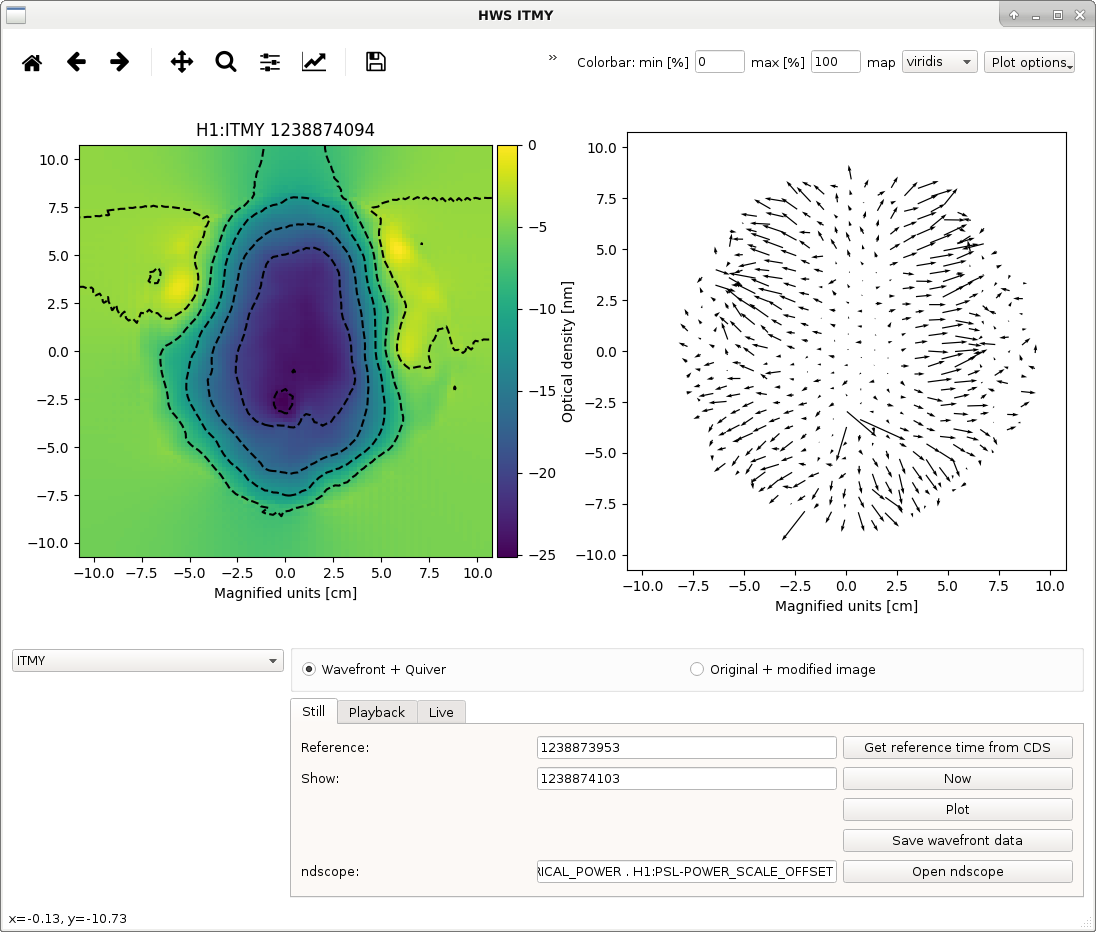
\includegraphics[width=\textwidth]{figs/TCS/PA/48349_20190409201649_inital_install_CO2Ymask2_150seconds_900mW.png}
%\caption{Point absorber figure with second $\mathrm{CO_2}$ mask}
%\label{fig:RH_power}
%\end{figure}

\end{itemize}

\section{Dynamic Thermal Compensation}
\subsection{A closer look at the ring heater / test mass thermo-optic response}
An analytical model of transient ring heater actuation from a radially symmetric thermal aberration ($\Psi(t,r)$) is realized \cite{Ramette:16}:
\begin{equation}
	\Psi(t,r)=2\frac{dn}{dT} \sum^{\infty}_{m,p = 1} A_{m,p} \; c^{u}_{p} \mathrm{sin}(u_m h /2a) (a/u_m)[1-e^{-\alpha t}] J_0(\zeta_p r/a)
\end{equation}

\begin{figure}[H]
 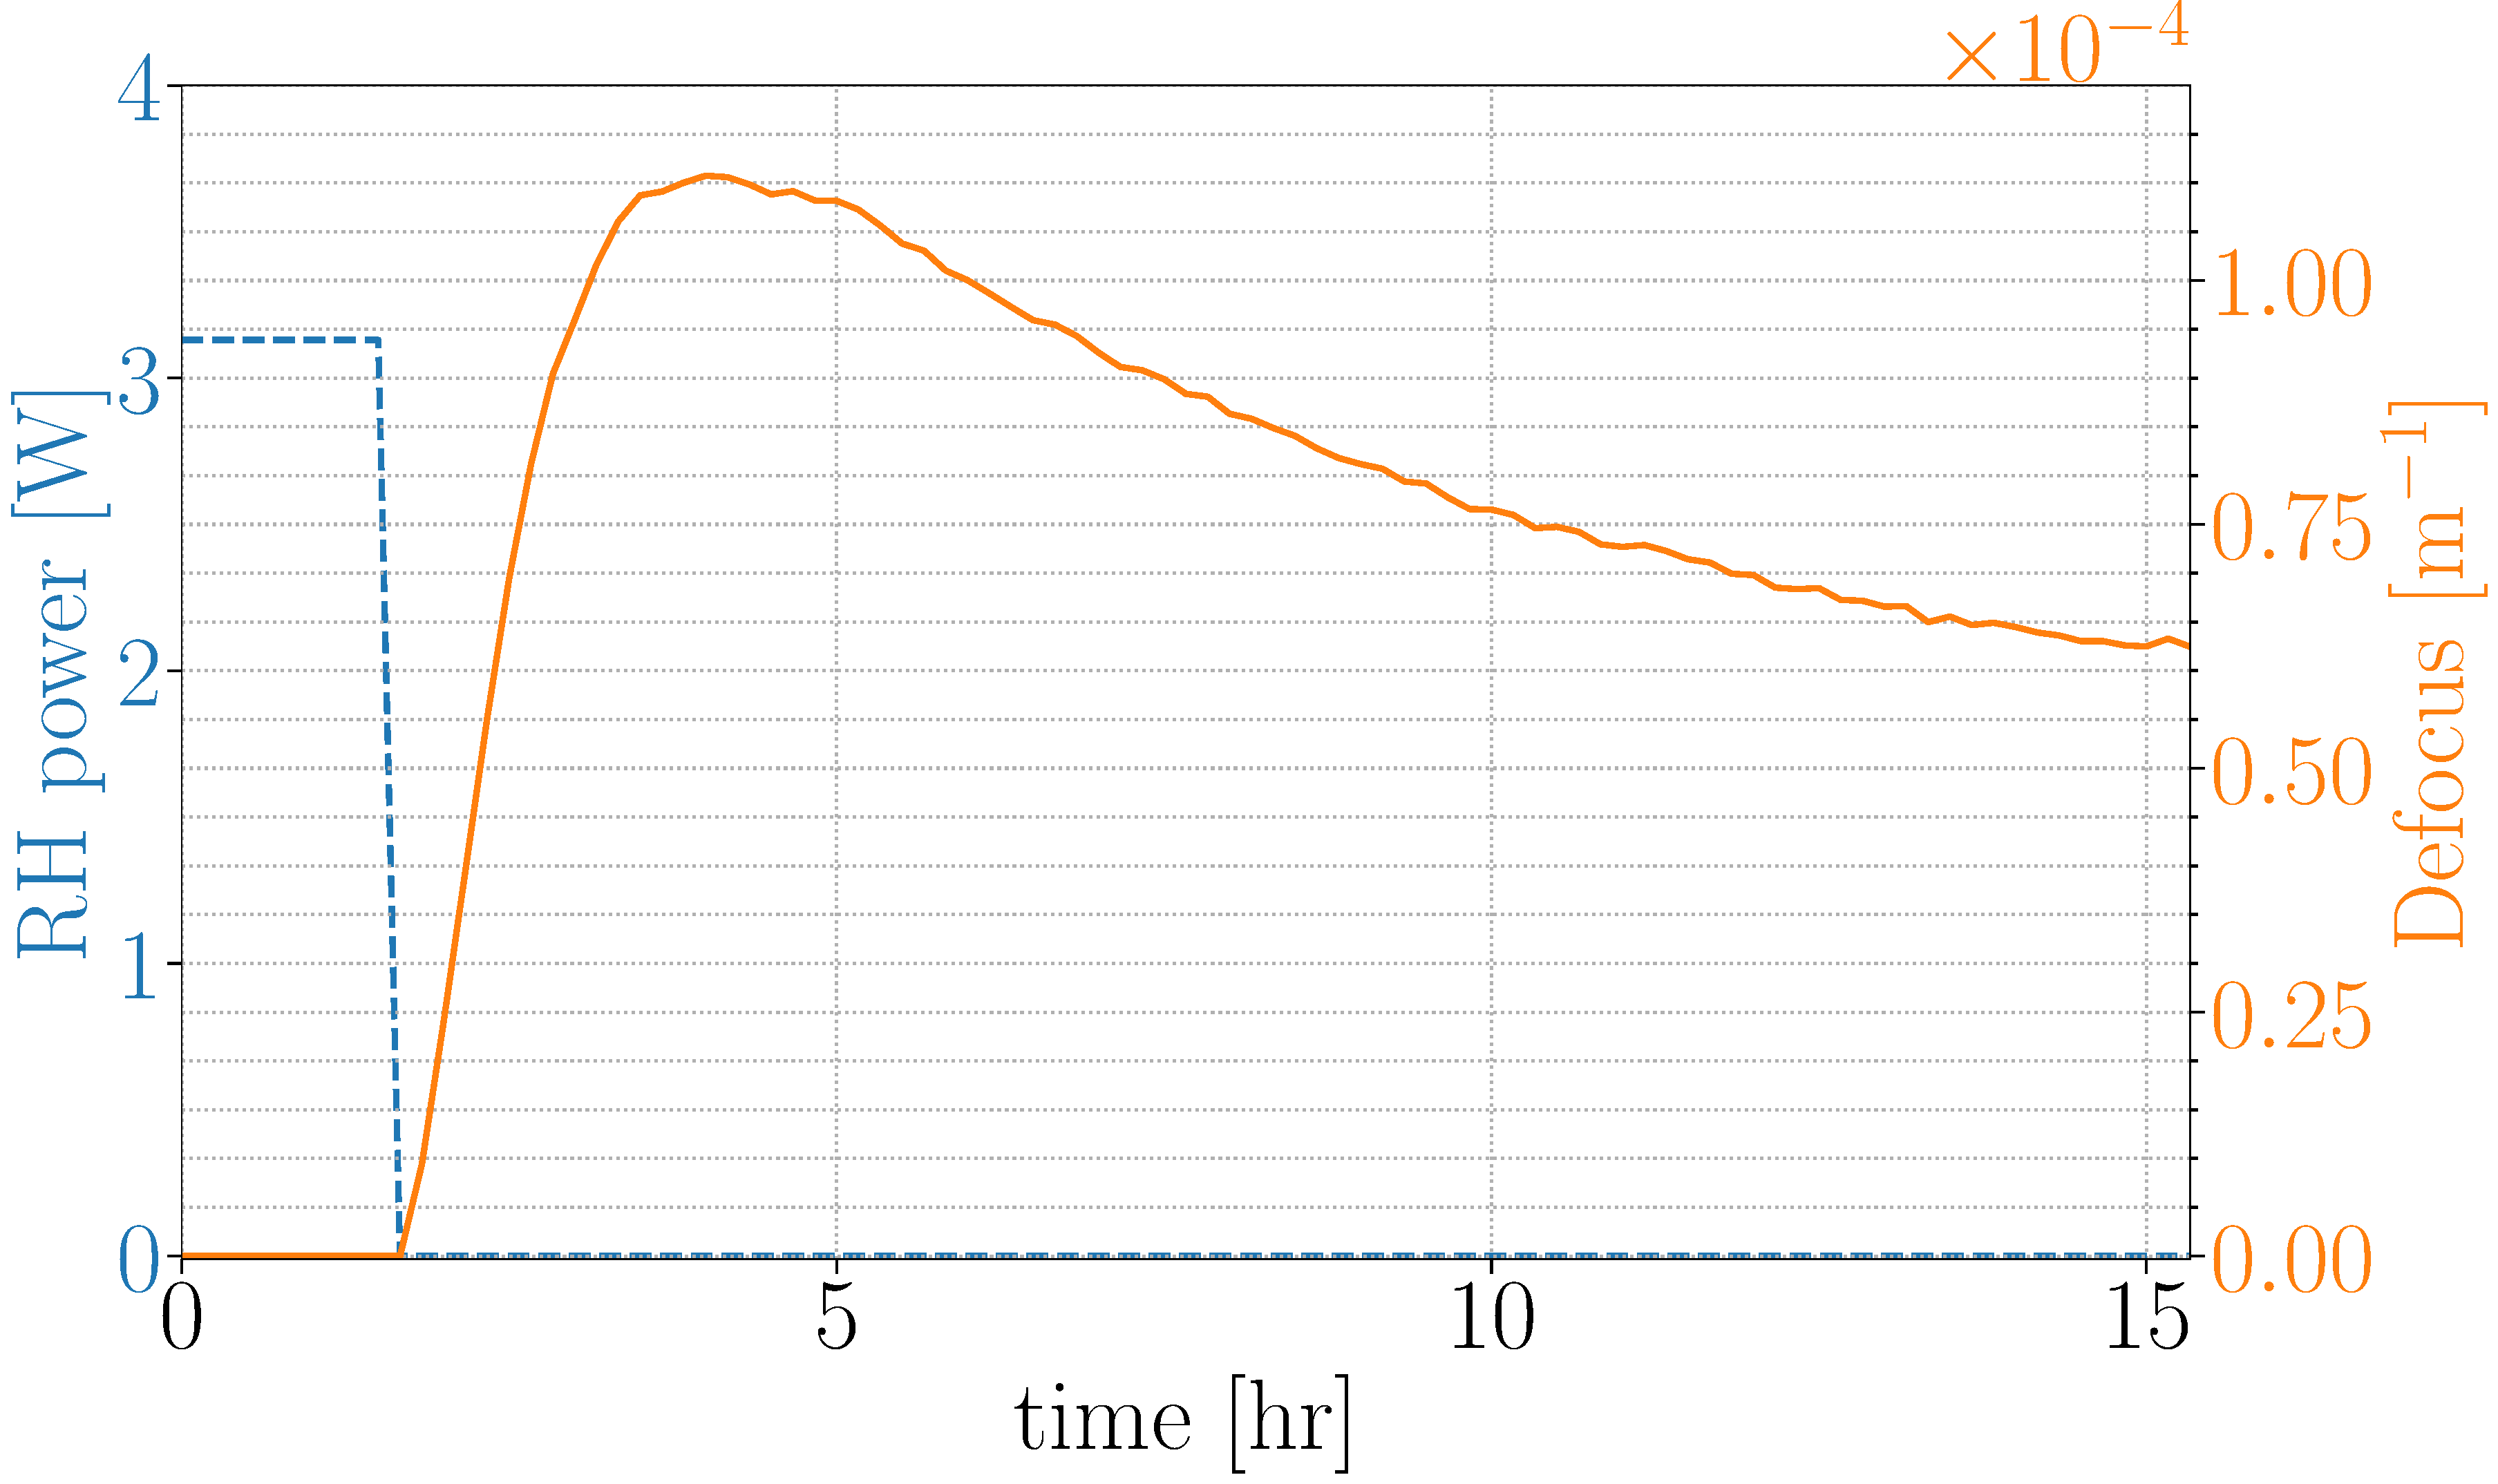
\includegraphics[width=\textwidth]{TCS/IRHF/Meas_response}
 \caption{ITMY thermo-optic response to a 3.13 Watt power reduction to the top and bottom ring heater elements. It's after $\approx$ 12 hours after the change was made do you start to see a small enough $\frac{\mathrm{d} \alpha_\mathrm{sp}}{\mathrm{dt}}$ when you can assume a steady thermal lens.}
 \label{fig:meas}
\end{figure}

The measured transient response exhibits a differential defocus on a time scale of $\approx$ 12 to 15 hours; stalling precious observing and/or detector comissioning time with differential mode matching for an extended period. Reducing the time constants for the differential defocus is possible though the construction and implementation of real time digital filtering applied to the ring heater power control input.

\begin{figure}[H]
\centering
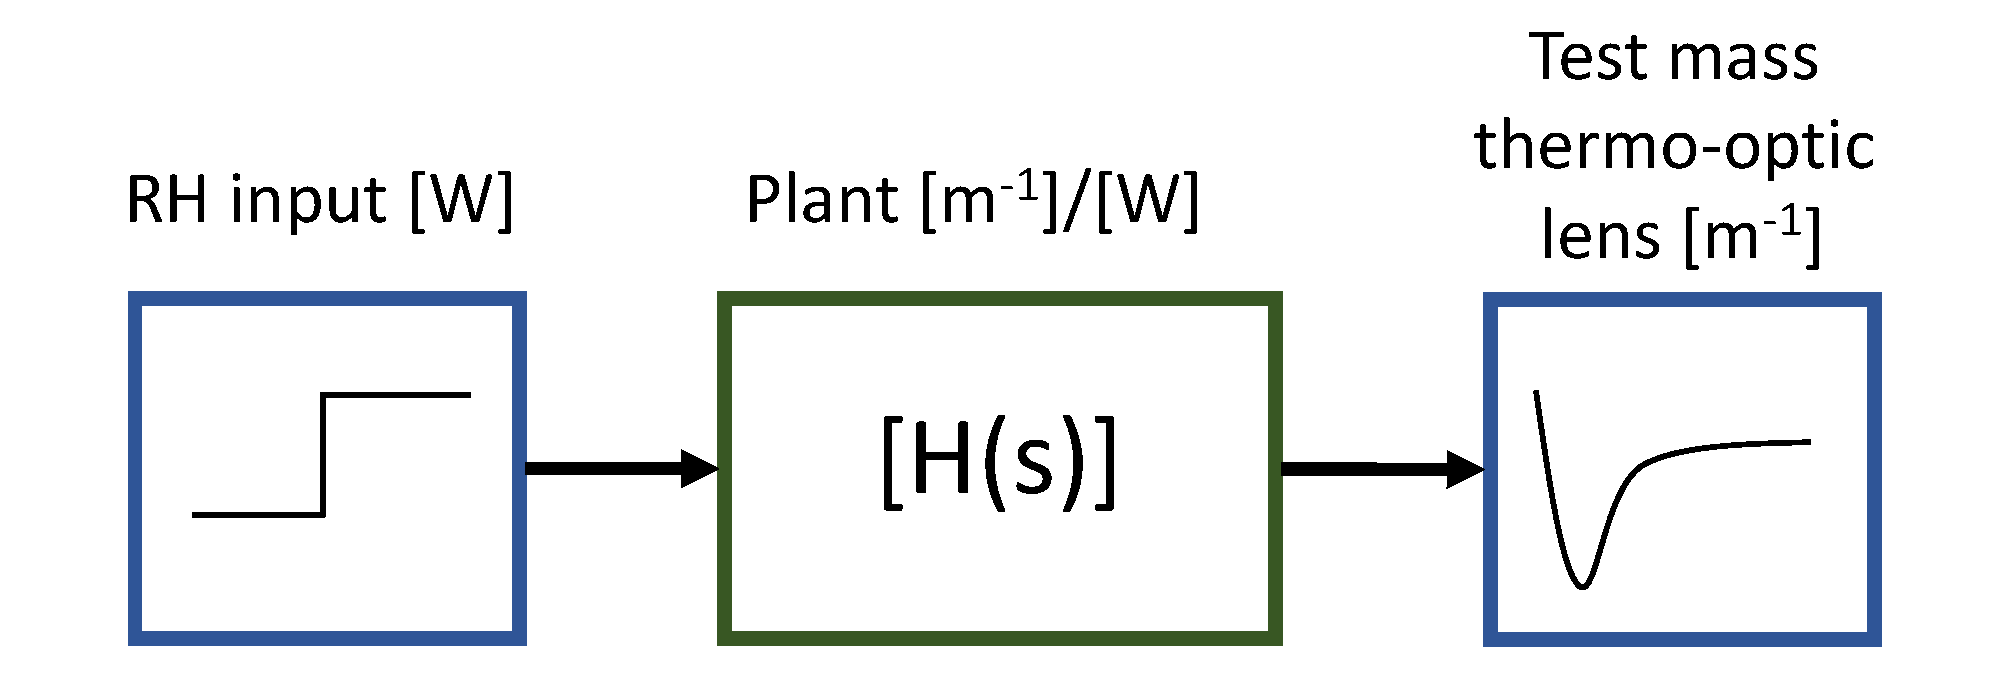
\includegraphics[page=1,width=.75\textwidth]{TCS/IRHF/RH_input_filter_figures.pdf}
\caption{A pictograph showing how the plant transforms the signal. The example of this can be seen in Fig [\ref{fig:meas}]}
\label{fig:justplant}
\end{figure}

The construction of the filter is realized with the following prescription:
\textcolor{red}{see appendix}
%\begin{enumerate}[label=\arabic*),leftmargin=75pt,nosep]
%	\item Fit step response to a zpk filter $H(s)$ 
%	\item Invert fitted filter ($H(s) \rightarrow H^{-1}(s)$) 
%	\item Apply correction filter $G(s)$ for stability and speed tuning ($H^{-1}(s)*G(s)$)
%\end{enumerate}


\begin{figure}[H]
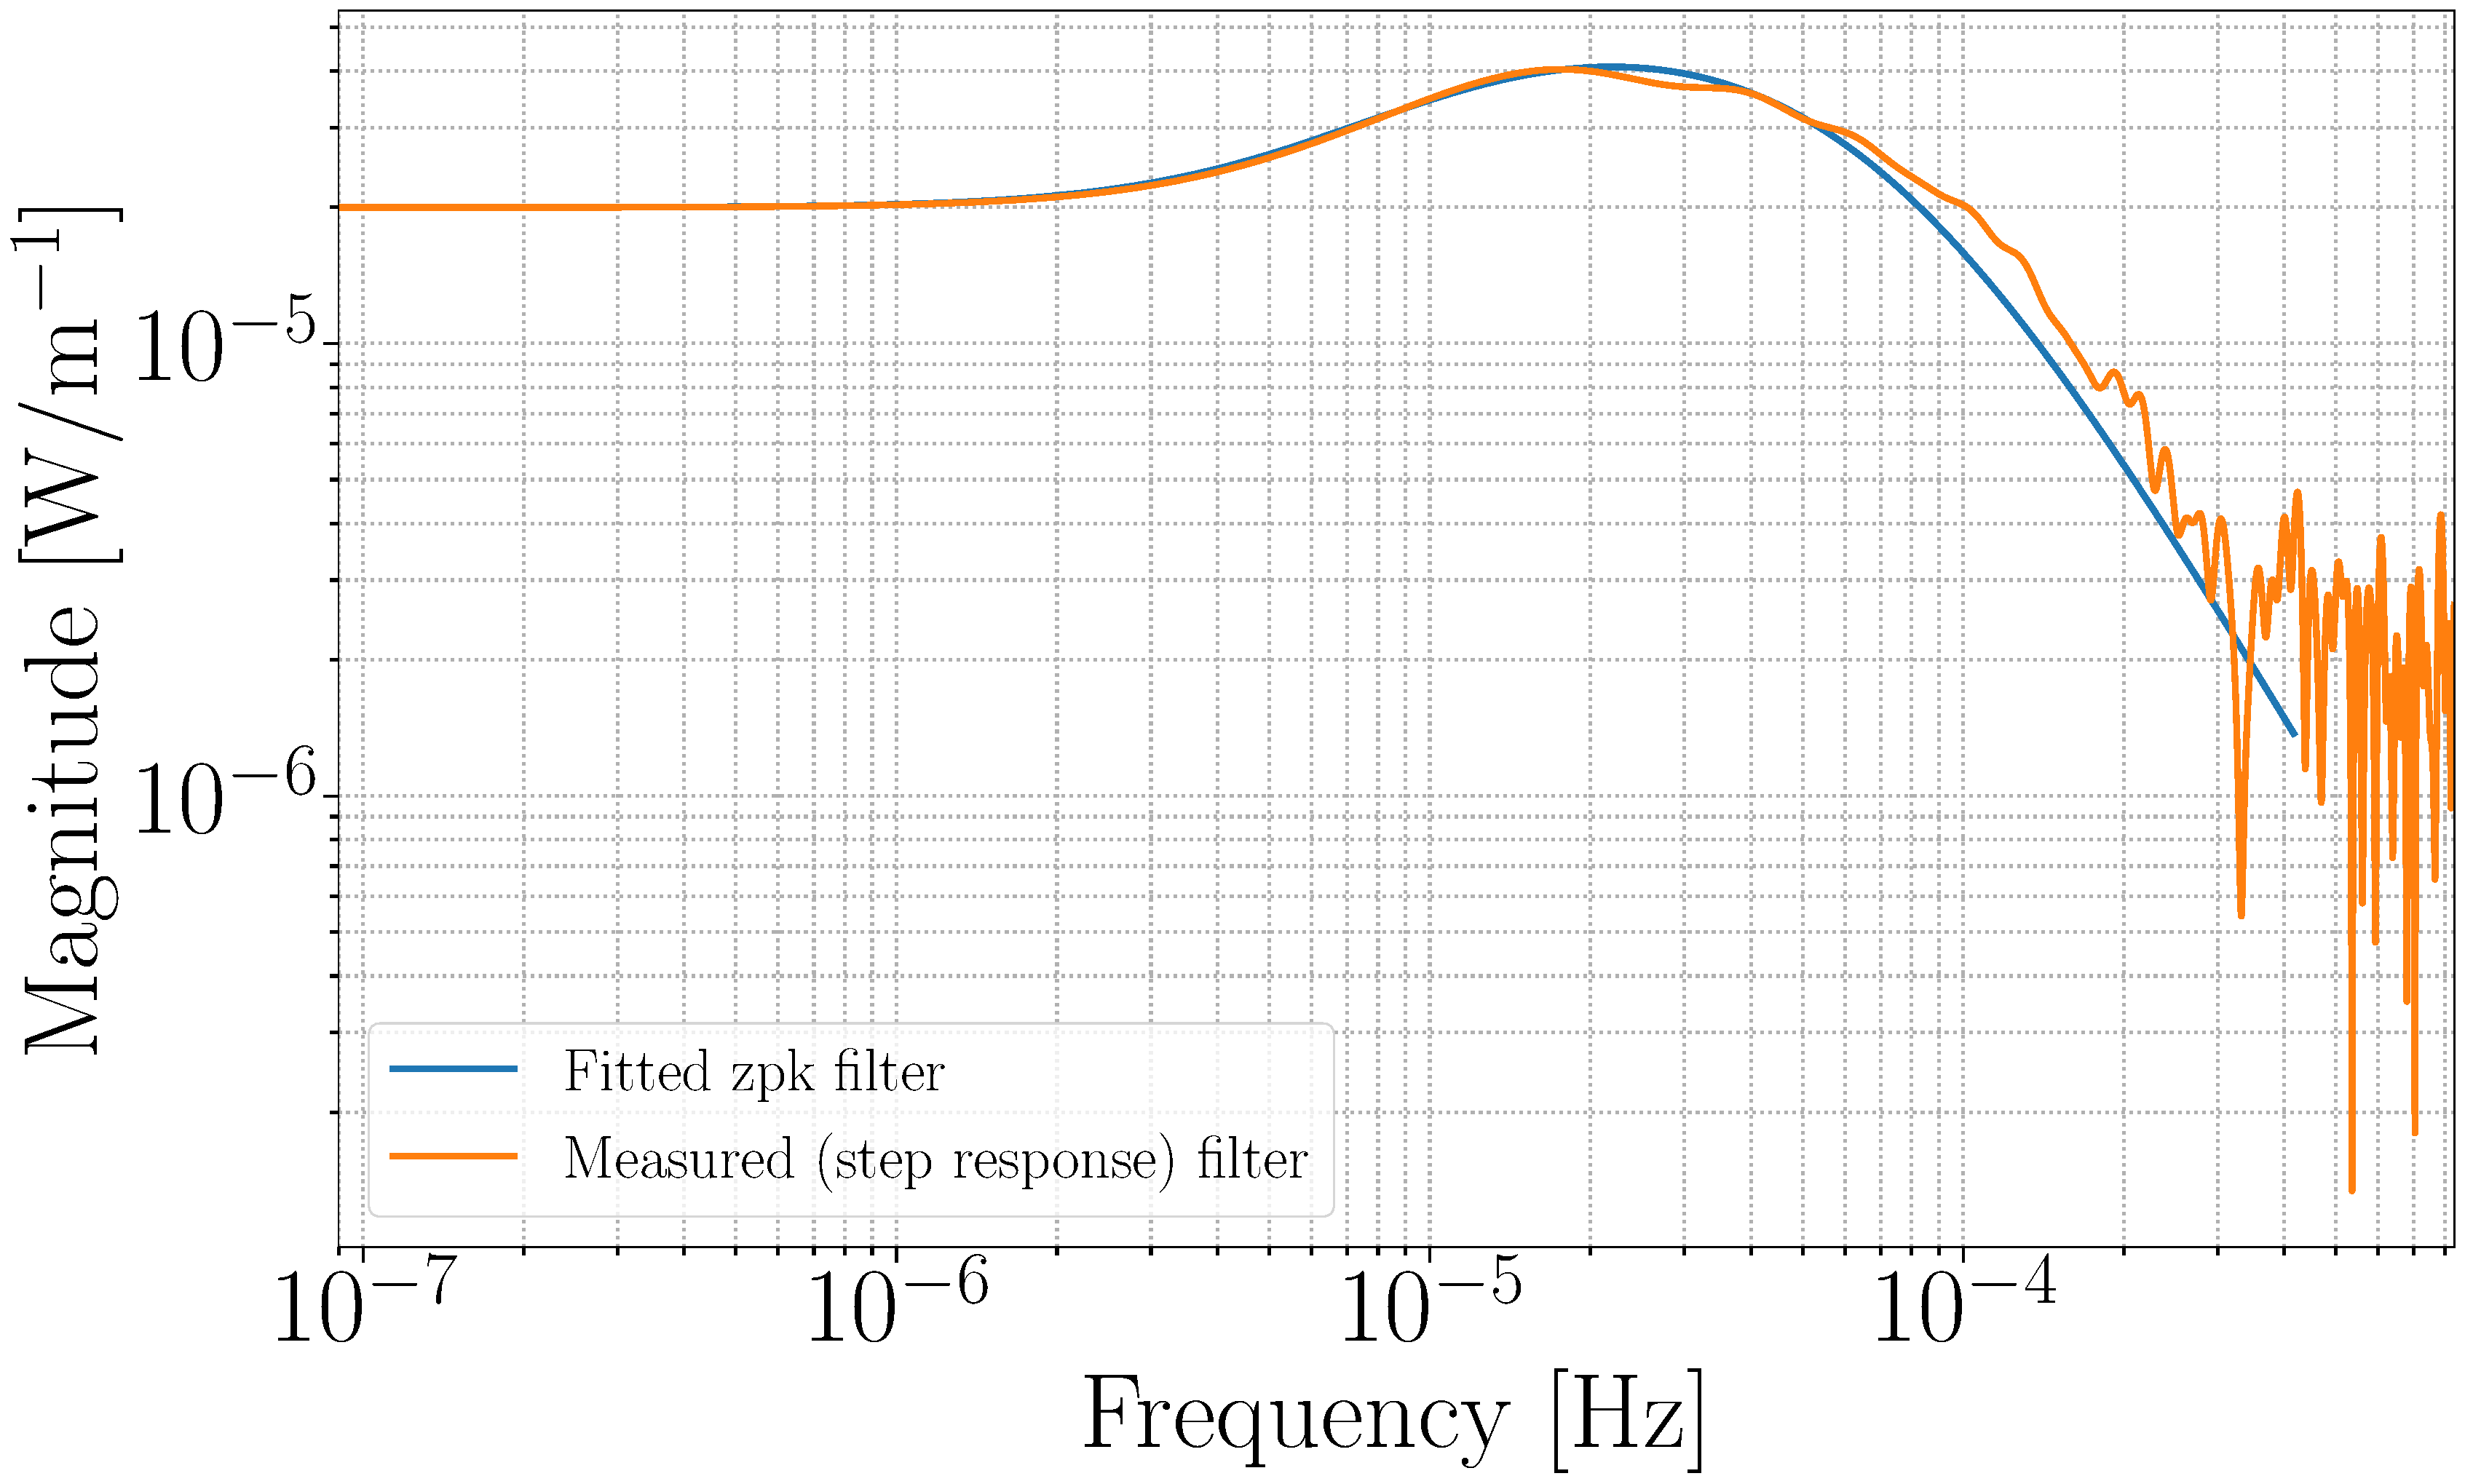
\includegraphics[width=\textwidth]{TCS/IRHF/RH_plant_filter_fit}
\caption{Showing the PSD of the RH response (normalized by the input RH power) over a an $\approx$ 12.5 hour period. The zpk model of the fitted filter (H(s)) is $9.2545e-12 \frac{(s+3.14210e-5)}{(s+8.168e-5)(s+0.0003142)(s+0.0005969)}$}
\label{fig:plant_v_fit}
\end{figure}

\begin{figure}[H]
\centering
\includegraphics[page=2,width=.9\textwidth]{TCS/IRHF/RH_input_filter_figures.pdf}
\caption{A pictograph showing the system with real time digital filtering for an improved thermo-optic response. The RH input filter is created by inverting the plant filter combine with a low pass and added poles to the zpk model to ensure stability.}
\label{fig:rtdf_pictograph}
\end{figure}

\begin{figure}[H]
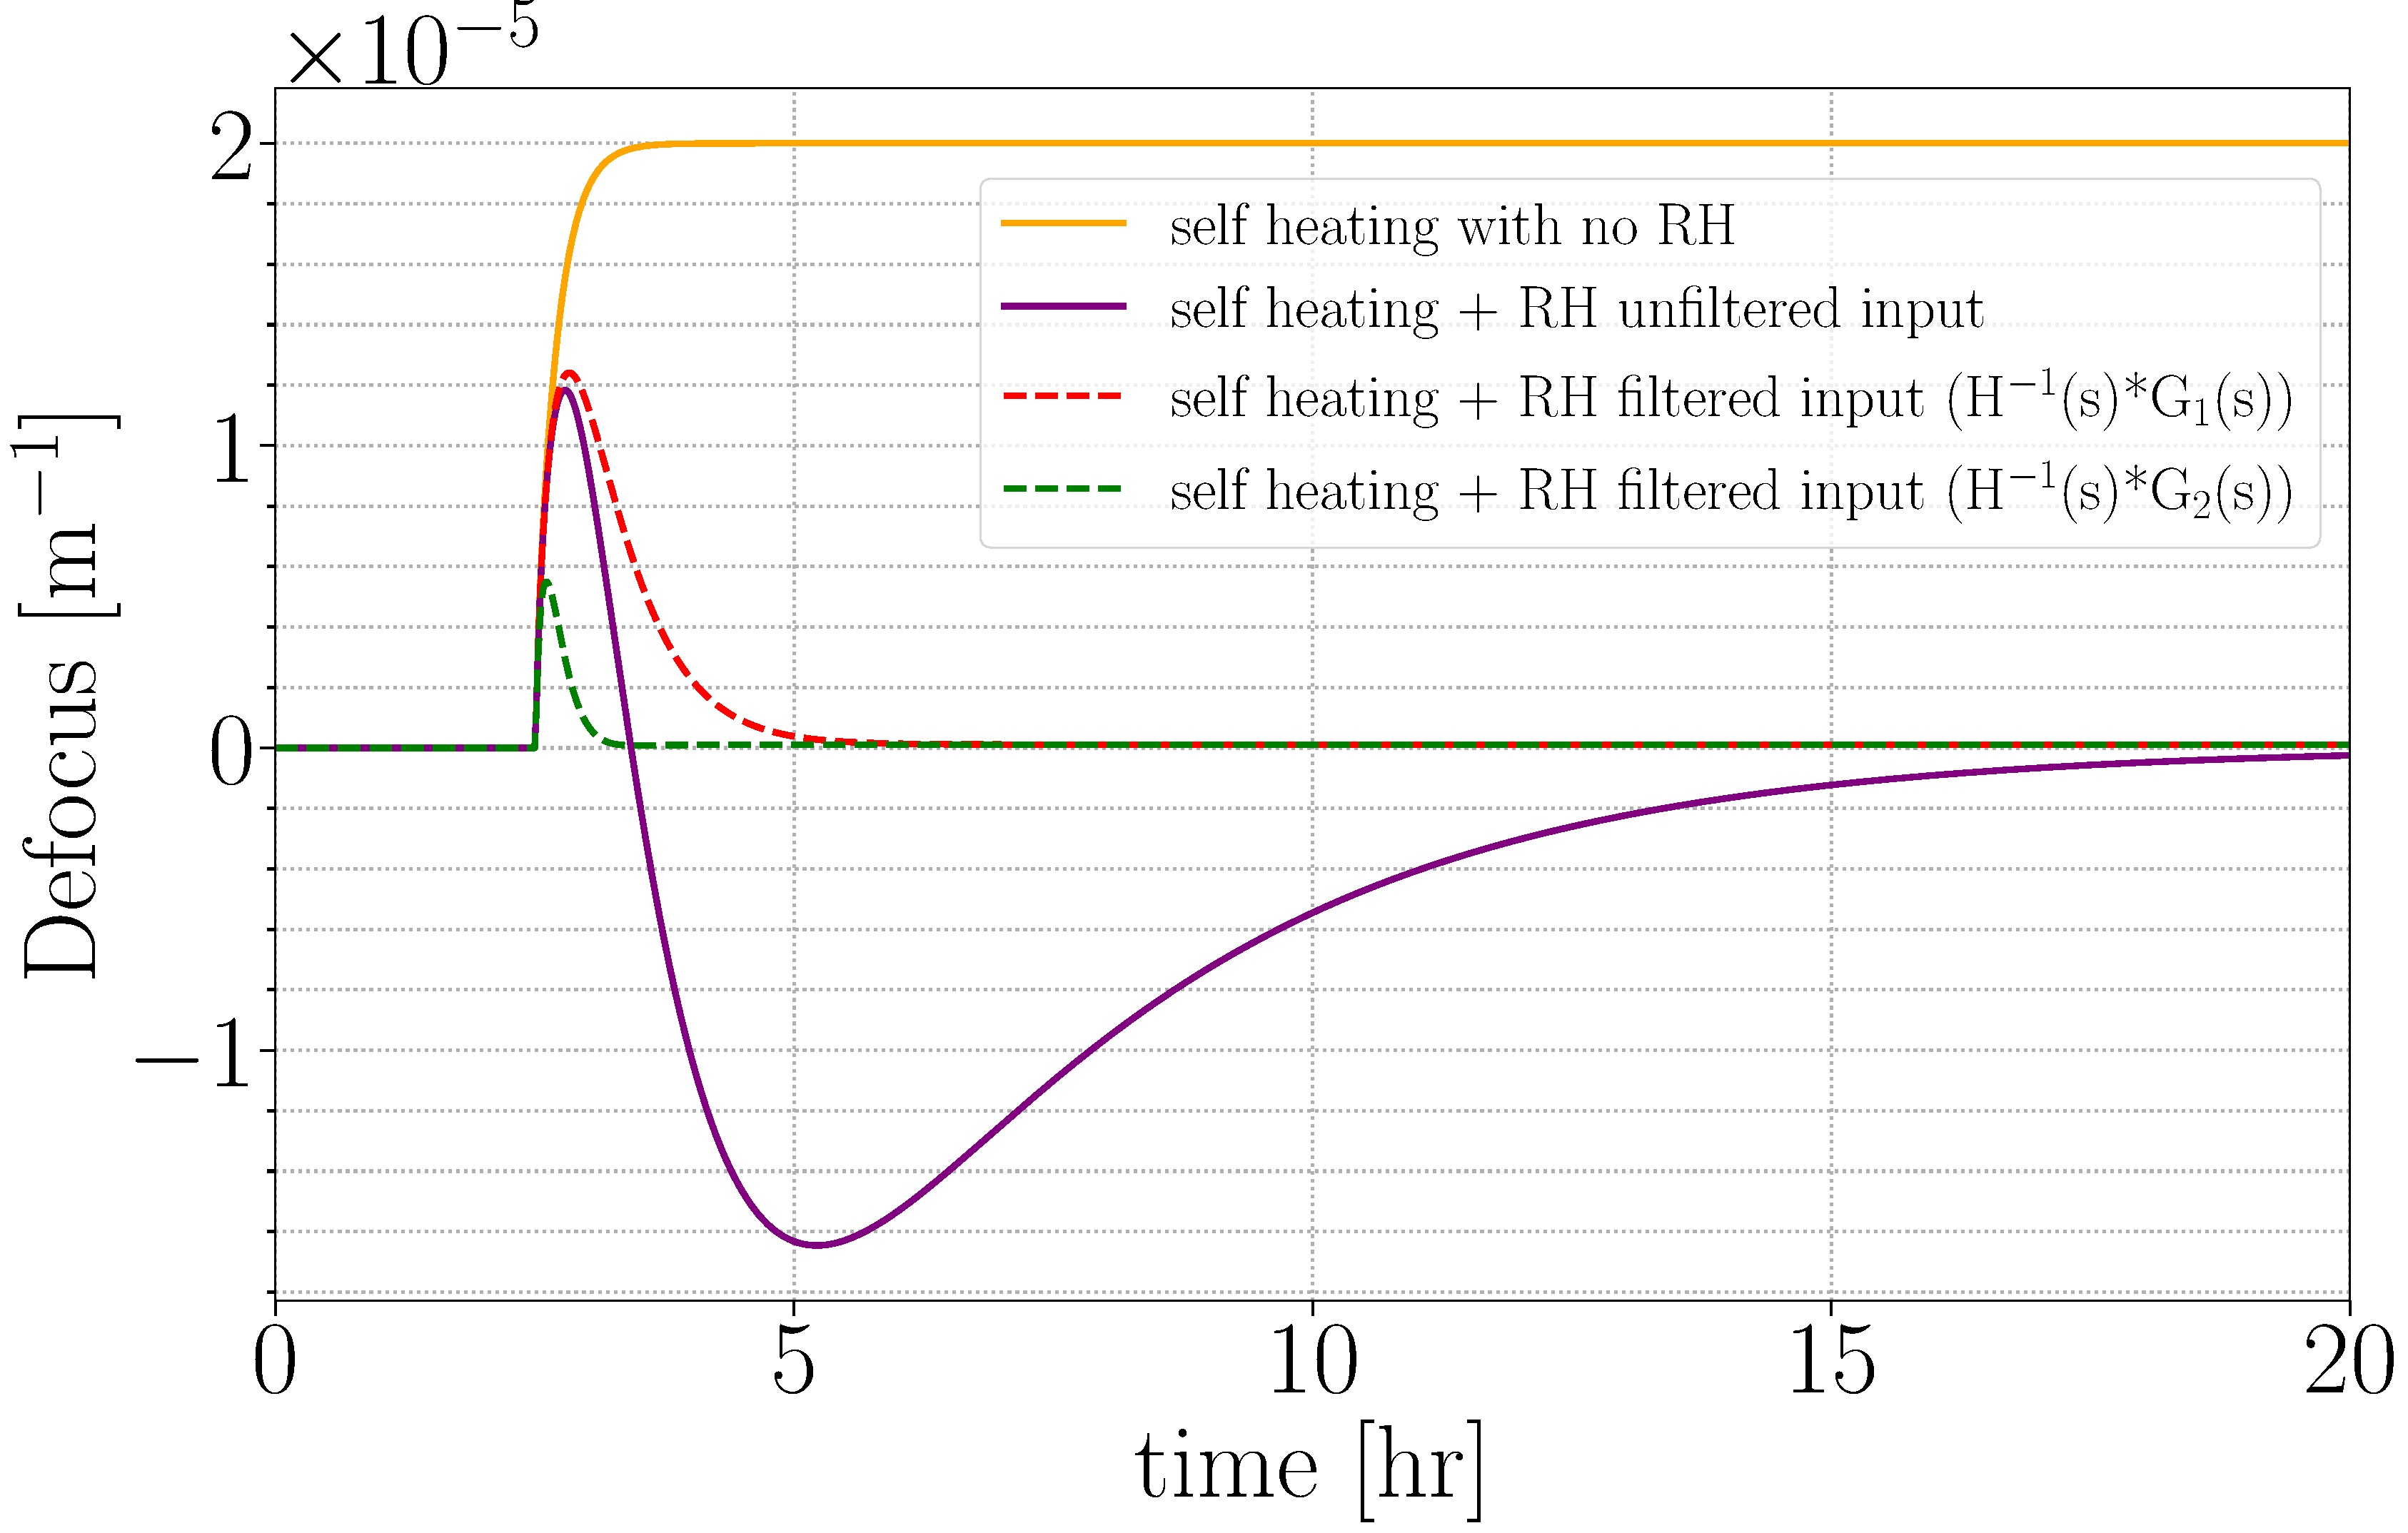
\includegraphics[width=\textwidth]{TCS/IRHF/IRHF_compare_w_self}
\caption{Comparison of the natural RH response and the response to the conditioned input. The above plot is simulated in Matlab by passing the RH input time series (top plot) through the $[H(s)]^{-1*}$ and $H(s)$ to acquire with the result lensing behavior on the bottom plot.}
\label{fig:dynam_comparison}
\end{figure}
\newpage

\subsubsection{Limitations}
\begin{figure}[H]
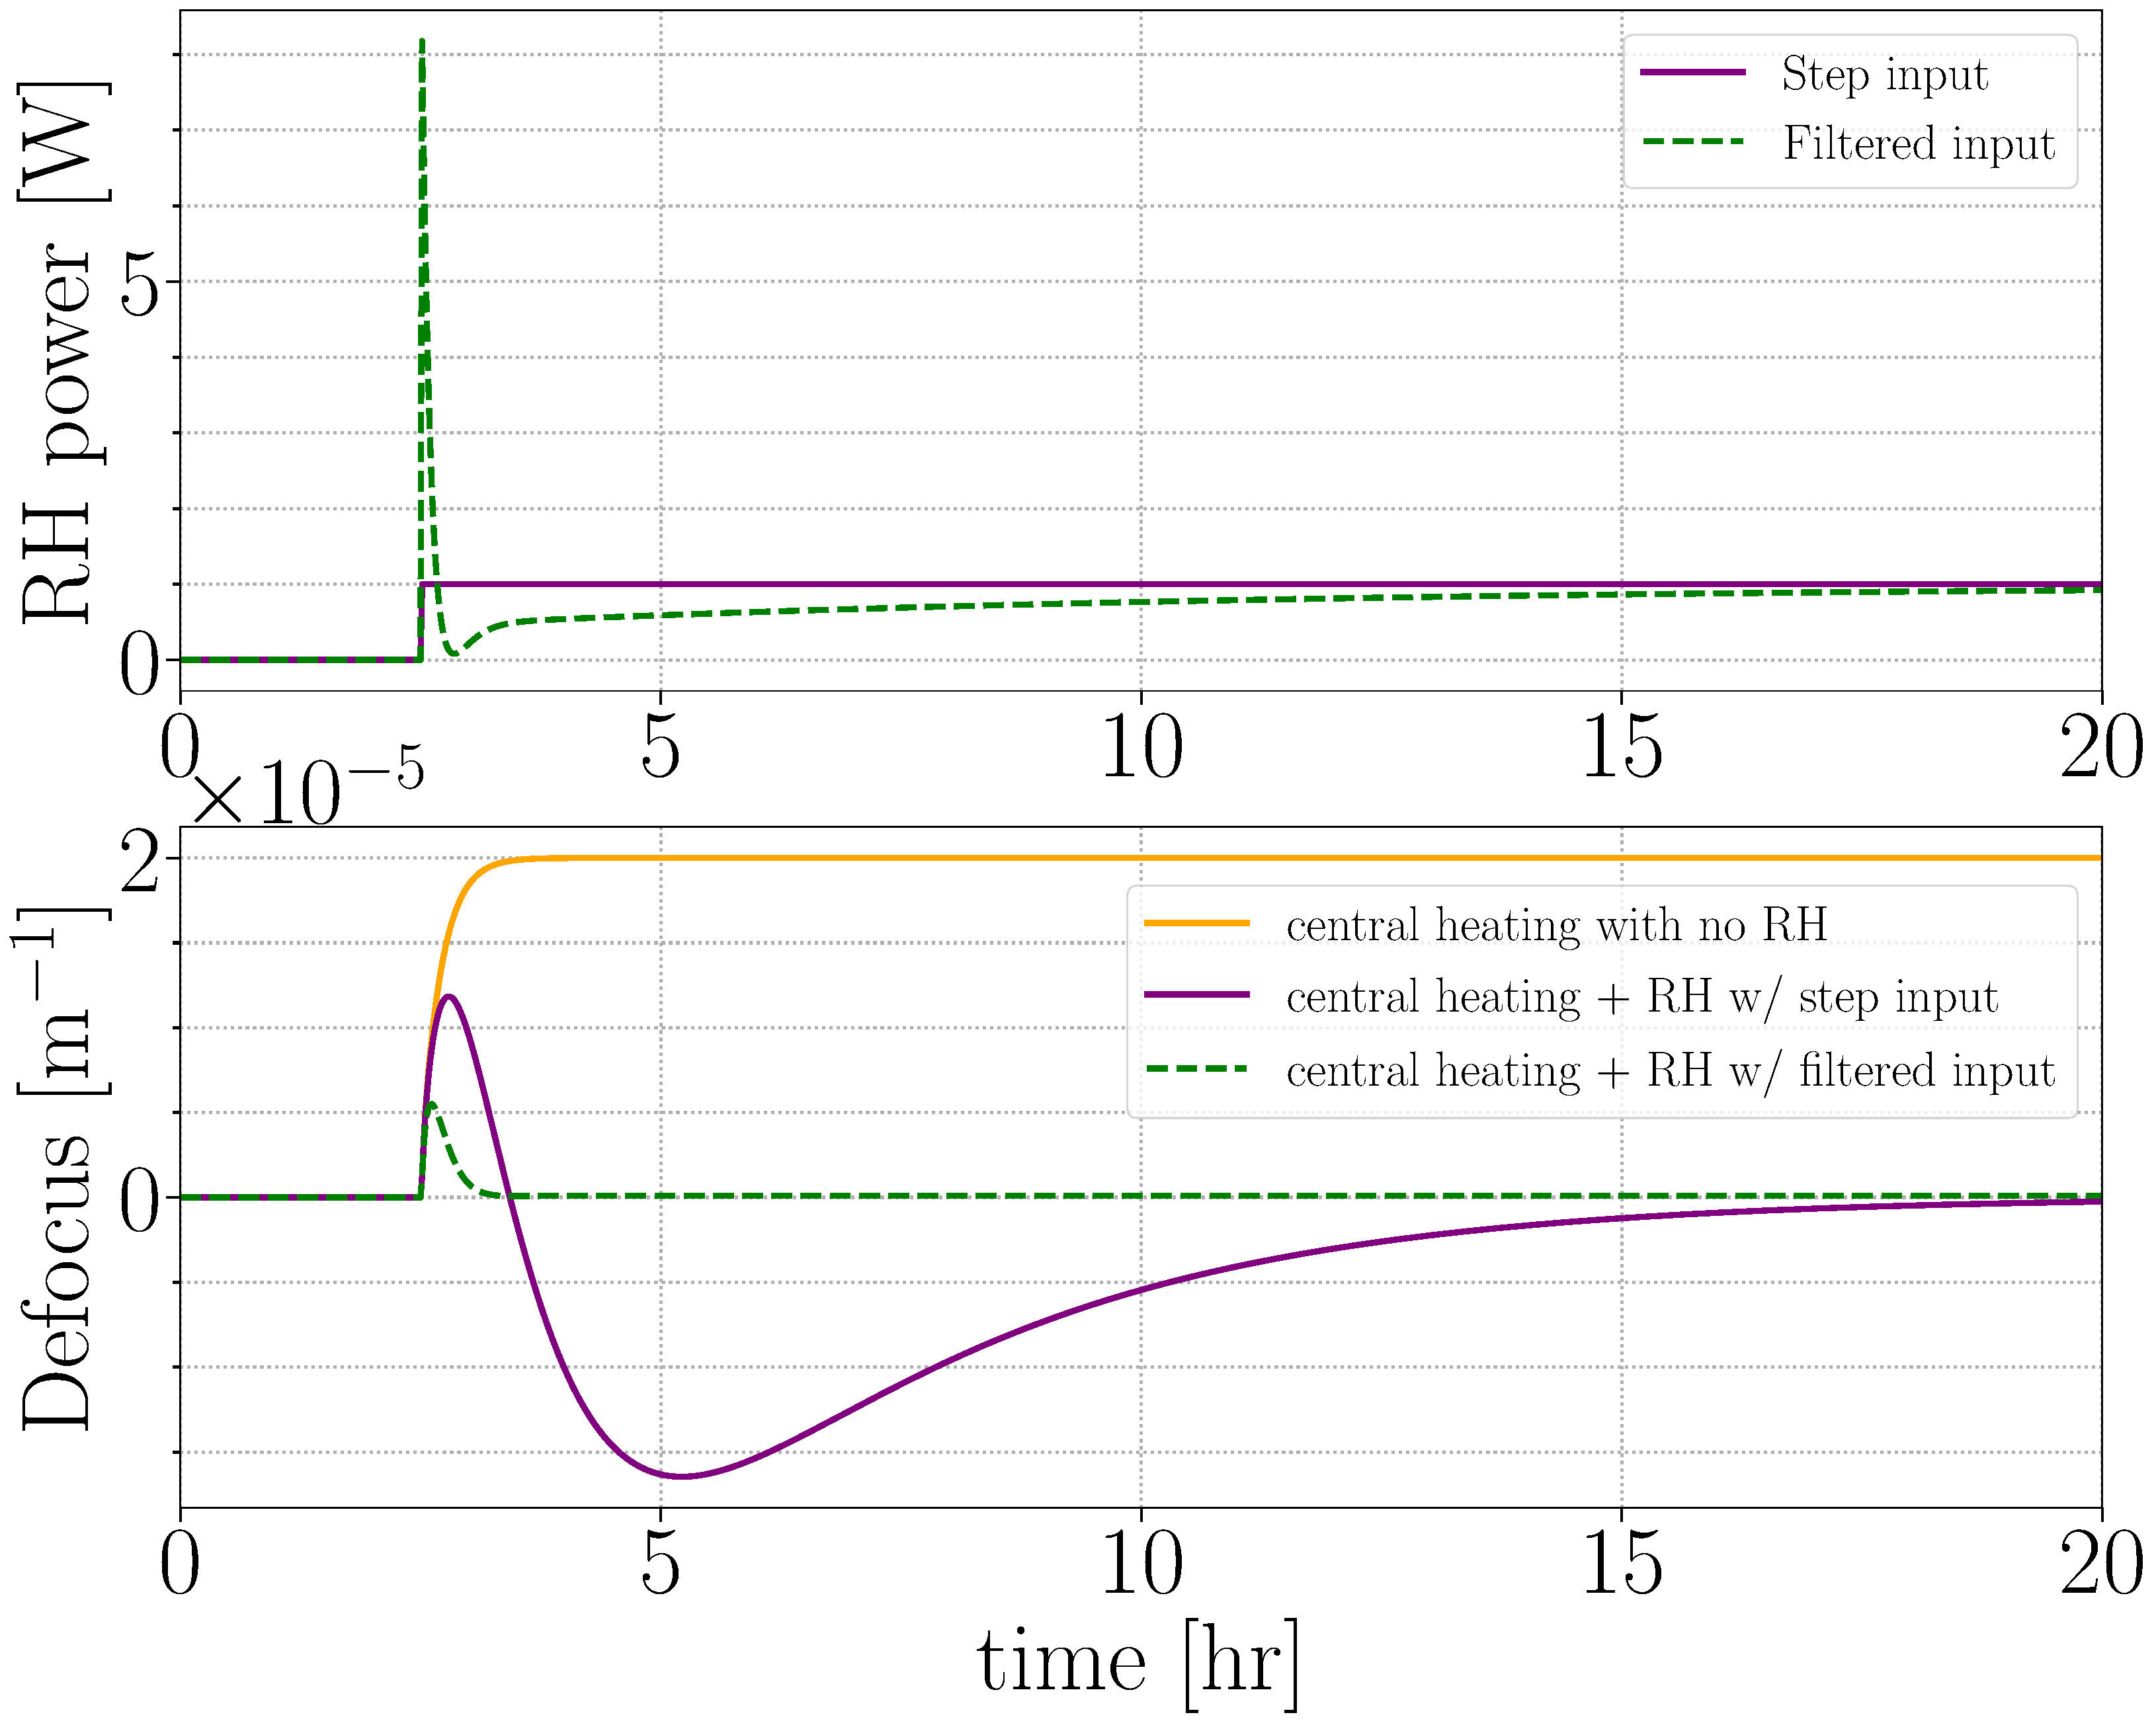
\includegraphics[width=\textwidth]{TCS/IRHF/IRHF_compare_filts_PI_paper}
\caption{Comparison of the natural RH response and the response to the filtered input with RH power}
\label{fig:RH_power}
\end{figure}
Limitation on RH power is set at 8W \textcolor{red}{Double check source?}

\textcolor{red}{Implementation into CDS at LHO (appendix?)}


